\documentclass[xcolor={table}]{beamer}
%\usetheme{singapore}
\usepackage{bm}
\usepackage{listings,verbatim}
\usepackage{fancyvrb,tikz,color,xcolor,colortbl}
%\usepackage[table]{xcolor}
%\usepackage{verbatim}
% \usepackage{array}
%\lstloadlanguages{R}
%\lstset{ language=R, basicstyle=\scriptsize\ttfamily, commentstyle=\ttfamily\color{gray}, numbers=left, numberstyle=\ttfamily\color{gray}\footnotesize, stepnumber=1, numbersep=5pt, backgroundcolor=\color{white}, showspaces=false, showstringspaces=false, showtabs=false, frame=single, tabsize=2, captionpos=b, breaklines=true, breakatwhitespace=false, escapeinside={}, keywordstyle={}, morekeywords={} }\renewcommand{\P}{\mathcal{P}}
%\newcommand{\bt}{\pmb{\theta}}
%\newcommand{\bG}{\pmb{\Gamma}}
\newcommand{\p}{\pause}
\definecolor{Grey}{rgb}{0.95,0.95,0.95}
\newcommand{\pitem}{\pause \item}
\newenvironment{graytext}{\color{gray}}{\ignorespacesafterend}

\newcommand\independent{\protect\mathpalette{\protect\independenT}{\perp}}
\def\independenT#1#2{\mathrel{\rlap{$#1#2$}\mkern2mu{#1#2}}}

\definecolor{umassblue}{RGB}{51,51,153}
\definecolor{umassgreen}{RGB}{0,102,102}
%\definecolor{blue}{RGB}{51,51,153}
\definecolor{bblue}{RGB}{0,0,255}
\definecolor{red}{RGB}{153,0,51}

\newcommand\verbbf[1]{\textcolor[RGB]{51,51,153}{\textbf{$\blacksquare$ #1}}}
\newcommand\verbrf[1]{\textcolor[RGB]{153,0,51}{\textbf{$\blacksquare$ #1}}}

\newcommand{\N}{\mathcal{N}}
\newcommand{\Y}{\bm{\mathcal{Y}}}

\usefonttheme{serif}

\newenvironment{changemargin}[2]{%
  \begin{list}{}{%
    \setlength{\topsep}{0pt}%
    \setlength{\leftmargin}{#1}%
    \setlength{\rightmargin}{#2}%
    \setlength{\listparindent}{\parindent}%
    \setlength{\itemindent}{\parindent}%
    \setlength{\parsep}{\parskip}%
  }%
  \item[]}{\end{list}}

%
\title{Inferring Latent Influence Diffusion Networks in The United States Senate}
%
\definecolor{umassred}{HTML}{8C2633}
\setbeamercolor{structure}{fg=umassblue}
\author{\Large\textbf{Matthew J. Denny}}

%\affil[1]{University of Massachusetts Amherst}
%\affil[2]{University of Connecticut}

\institute{\Large Penn State University ---
 \texttt{mzd5530@psu.edu}\\
 \color{blue}\texttt{www.mjdenny.com}\\
 \texttt{@MatthewJDenny}
}

\date{ \today }
\begin{document}


% \begin{frame}
%   \titlepage
% \end{frame}






\begin{frame}\frametitle{Hierarchy in Networks--Datasets}
	\LARGE
\begin{itemize}
	\item Manager to Manager Email Data
	\vspace{.2in}
	\begin{itemize}
		\Large
		\item County manager should be at top of hierarchy.
	\end{itemize}
	\vspace{.2in}

	\item Congressional Influence
	\vspace{.2in}
	\begin{itemize}
		\Large
		\item Party leaders should be at the top of hierarchy.
	\end{itemize}
	\item Many More...
\end{itemize}
\end{frame}

\begin{frame}\frametitle{Hierarchy in networks--Measures}
\begin{table}
	\begin{tabular}{| r || c | c | c | c |}
		\hline
		Measure & Undirected & Weighted & Global & Local \\
		\hline
		Landau's h & & X& X& \\
		Kendall's K & X& X& &X\\
		Reach Degree & X& X& &X\\
		Reach Closeness & X& X& &X\\
		GRC & X& X& X&X\\
		Rooted Depth & & & X&\\
		Degree & X& X& X&X\\
		Closeness & X& X& X&X\\
		Betweenness & X& X& X&X\\
		Eigenvector &  X& X& X& X \\
		\hline
	\end{tabular}
\end{table}
\end{frame}

\begin{frame}\frametitle{Hierarchy in Networks -- Global Measures}
\begin{changemargin}{-2cm}{ -2cm}
	\centering
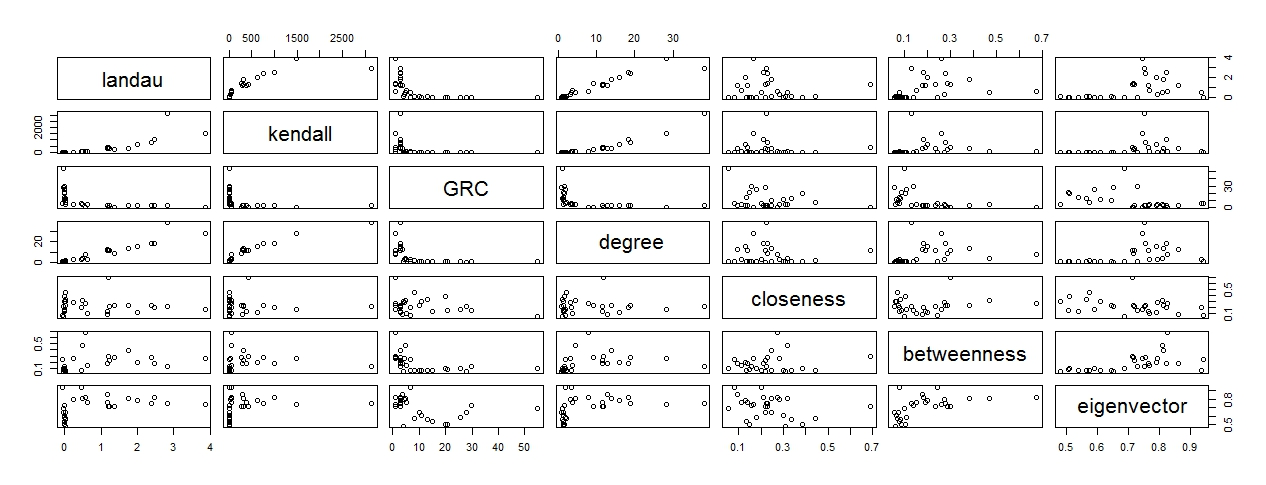
\includegraphics[scale = 0.3]{images/pairs_global.jpeg}
\end{changemargin}
\tiny
*Measures for all 29 datasets.
\end{frame}

\begin{frame}\frametitle{Hierarchy in Networks -- Local Measures}
	\begin{changemargin}{-2cm}{ -2cm}
		\centering
		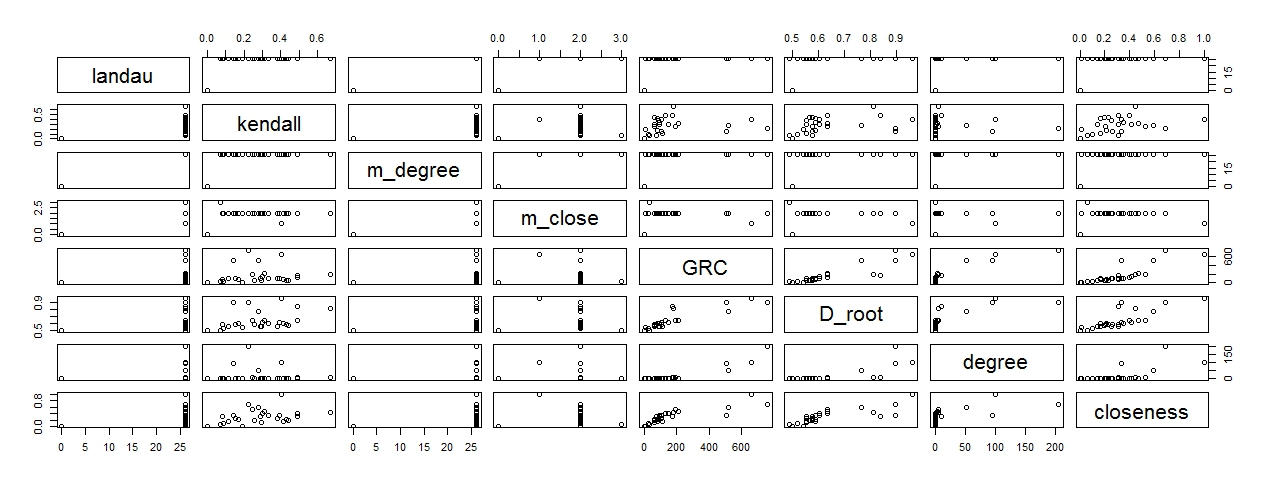
\includegraphics[scale = 0.3]{images/pairs_local.jpeg}
	\end{changemargin}
	\tiny
	*Measures for dataset 6.
\end{frame}

\begin{frame}\frametitle{Hierarchy in Networks -- Comparing Measures}
\begin{changemargin}{-2cm}{ -2cm}
	\centering
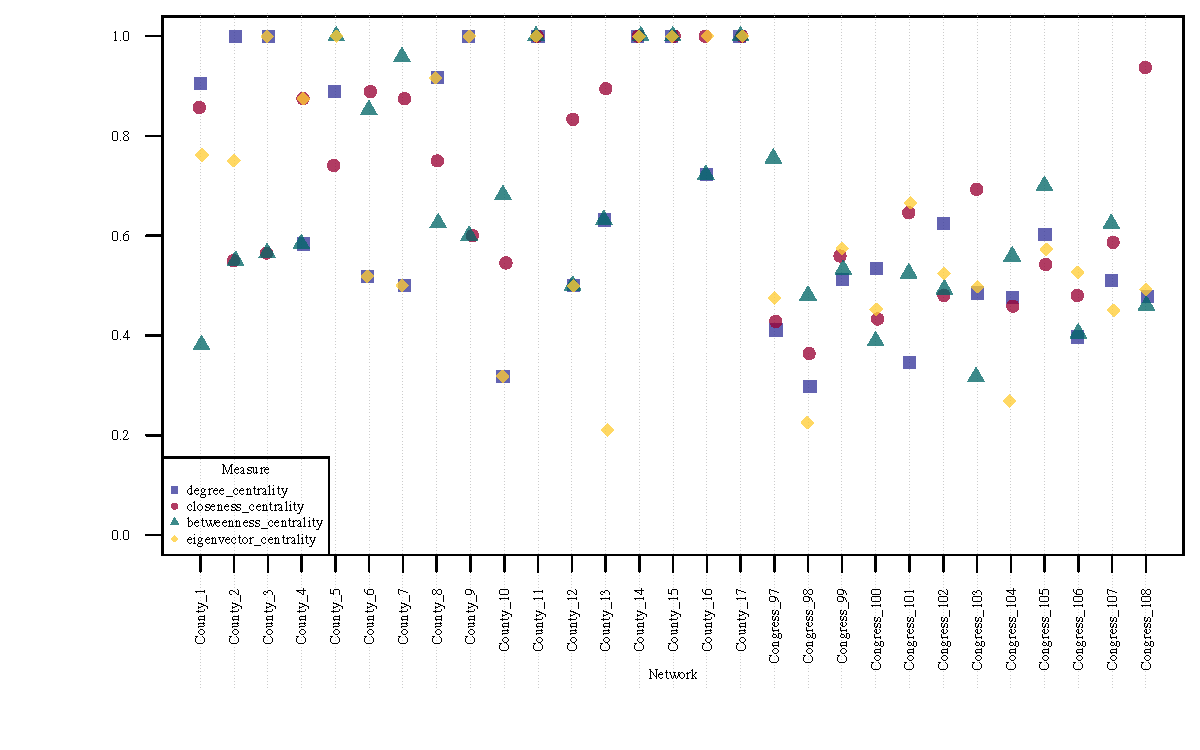
\includegraphics[scale = 0.65]{images/Measure_Scores.pdf}
\end{changemargin}
\end{frame}

\begin{frame}\frametitle{Hiearchy in Networks -- PCA}
\begin{changemargin}{-2cm}{ -2cm}
\begin{tikzpicture}
    \node(a) at (8,4){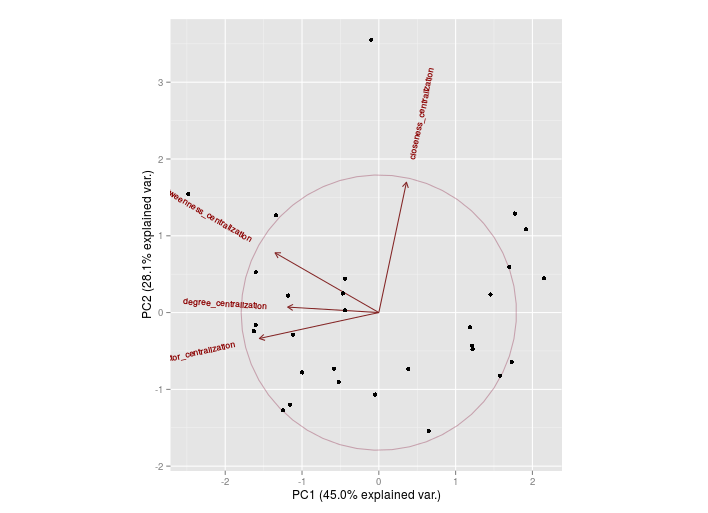
\includegraphics[width=13cm, height=8cm]{images/pca_biplot}};
    \pause
    \node(b) at (12.5,6.5){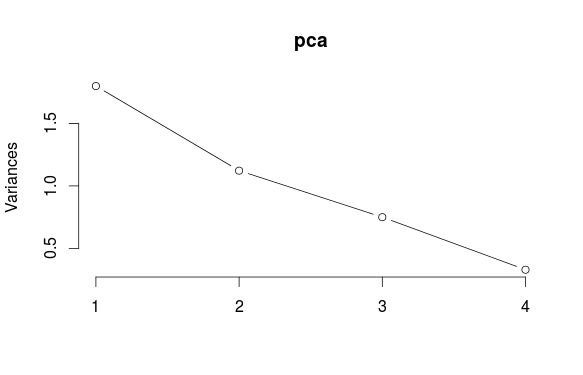
\includegraphics[width=4cm]{images/pca_variance}};
    \draw[blue,->](11.1,5.6)--(8,0.5);
    \draw[blue,->](12,5.5)--(4.5,4);
  \end{tikzpicture}
\end{changemargin}
\end{frame}

\end{document}
